\label{chp:b3}

Image fusion can be decomposed into three key components: the feature extractor, feature fuser, and image reconstructor. The feature extractor is responsible for extracting multilevel features from input images. Subsequently, the feature fuser amalgamates these extracted features into unified feature maps for each level. These consolidated features play a crucial role in the final image reconstruction, orchestrated by the image reconstructor.

In terms of analogy, the feature extractor corresponds to the encoder in autoencoders, while the image reconstructor aligns with the decoder in autoencoders. The feature fuser leverages both Convolutional Neural Networks (CNNs) and transformers, with CNNs adeptly managing local features and transformers overseeing global contexts. This amalgamation enhances the fusion process, ultimately aiming to improve accuracy.

Our approach involves a two-stage training process. In the initial stage, we train an autoencoder, originally derived from RFN-Nest \cite{li2021rfn} as illustrated in Figure \ref{fig:ch3:rfnnest}. Subsequently, in the second stage, we train our fusion block, depicted in Figure \ref{fig:fusionblock}, in conjunction with the previously trained autoencoder.

\subsection{Stage 1: Autoencoder Selection} \label{subsec:aesel}

\begin{figure}[htbp]
    \centering
    \begin{subfigure}[b]{\textwidth}
        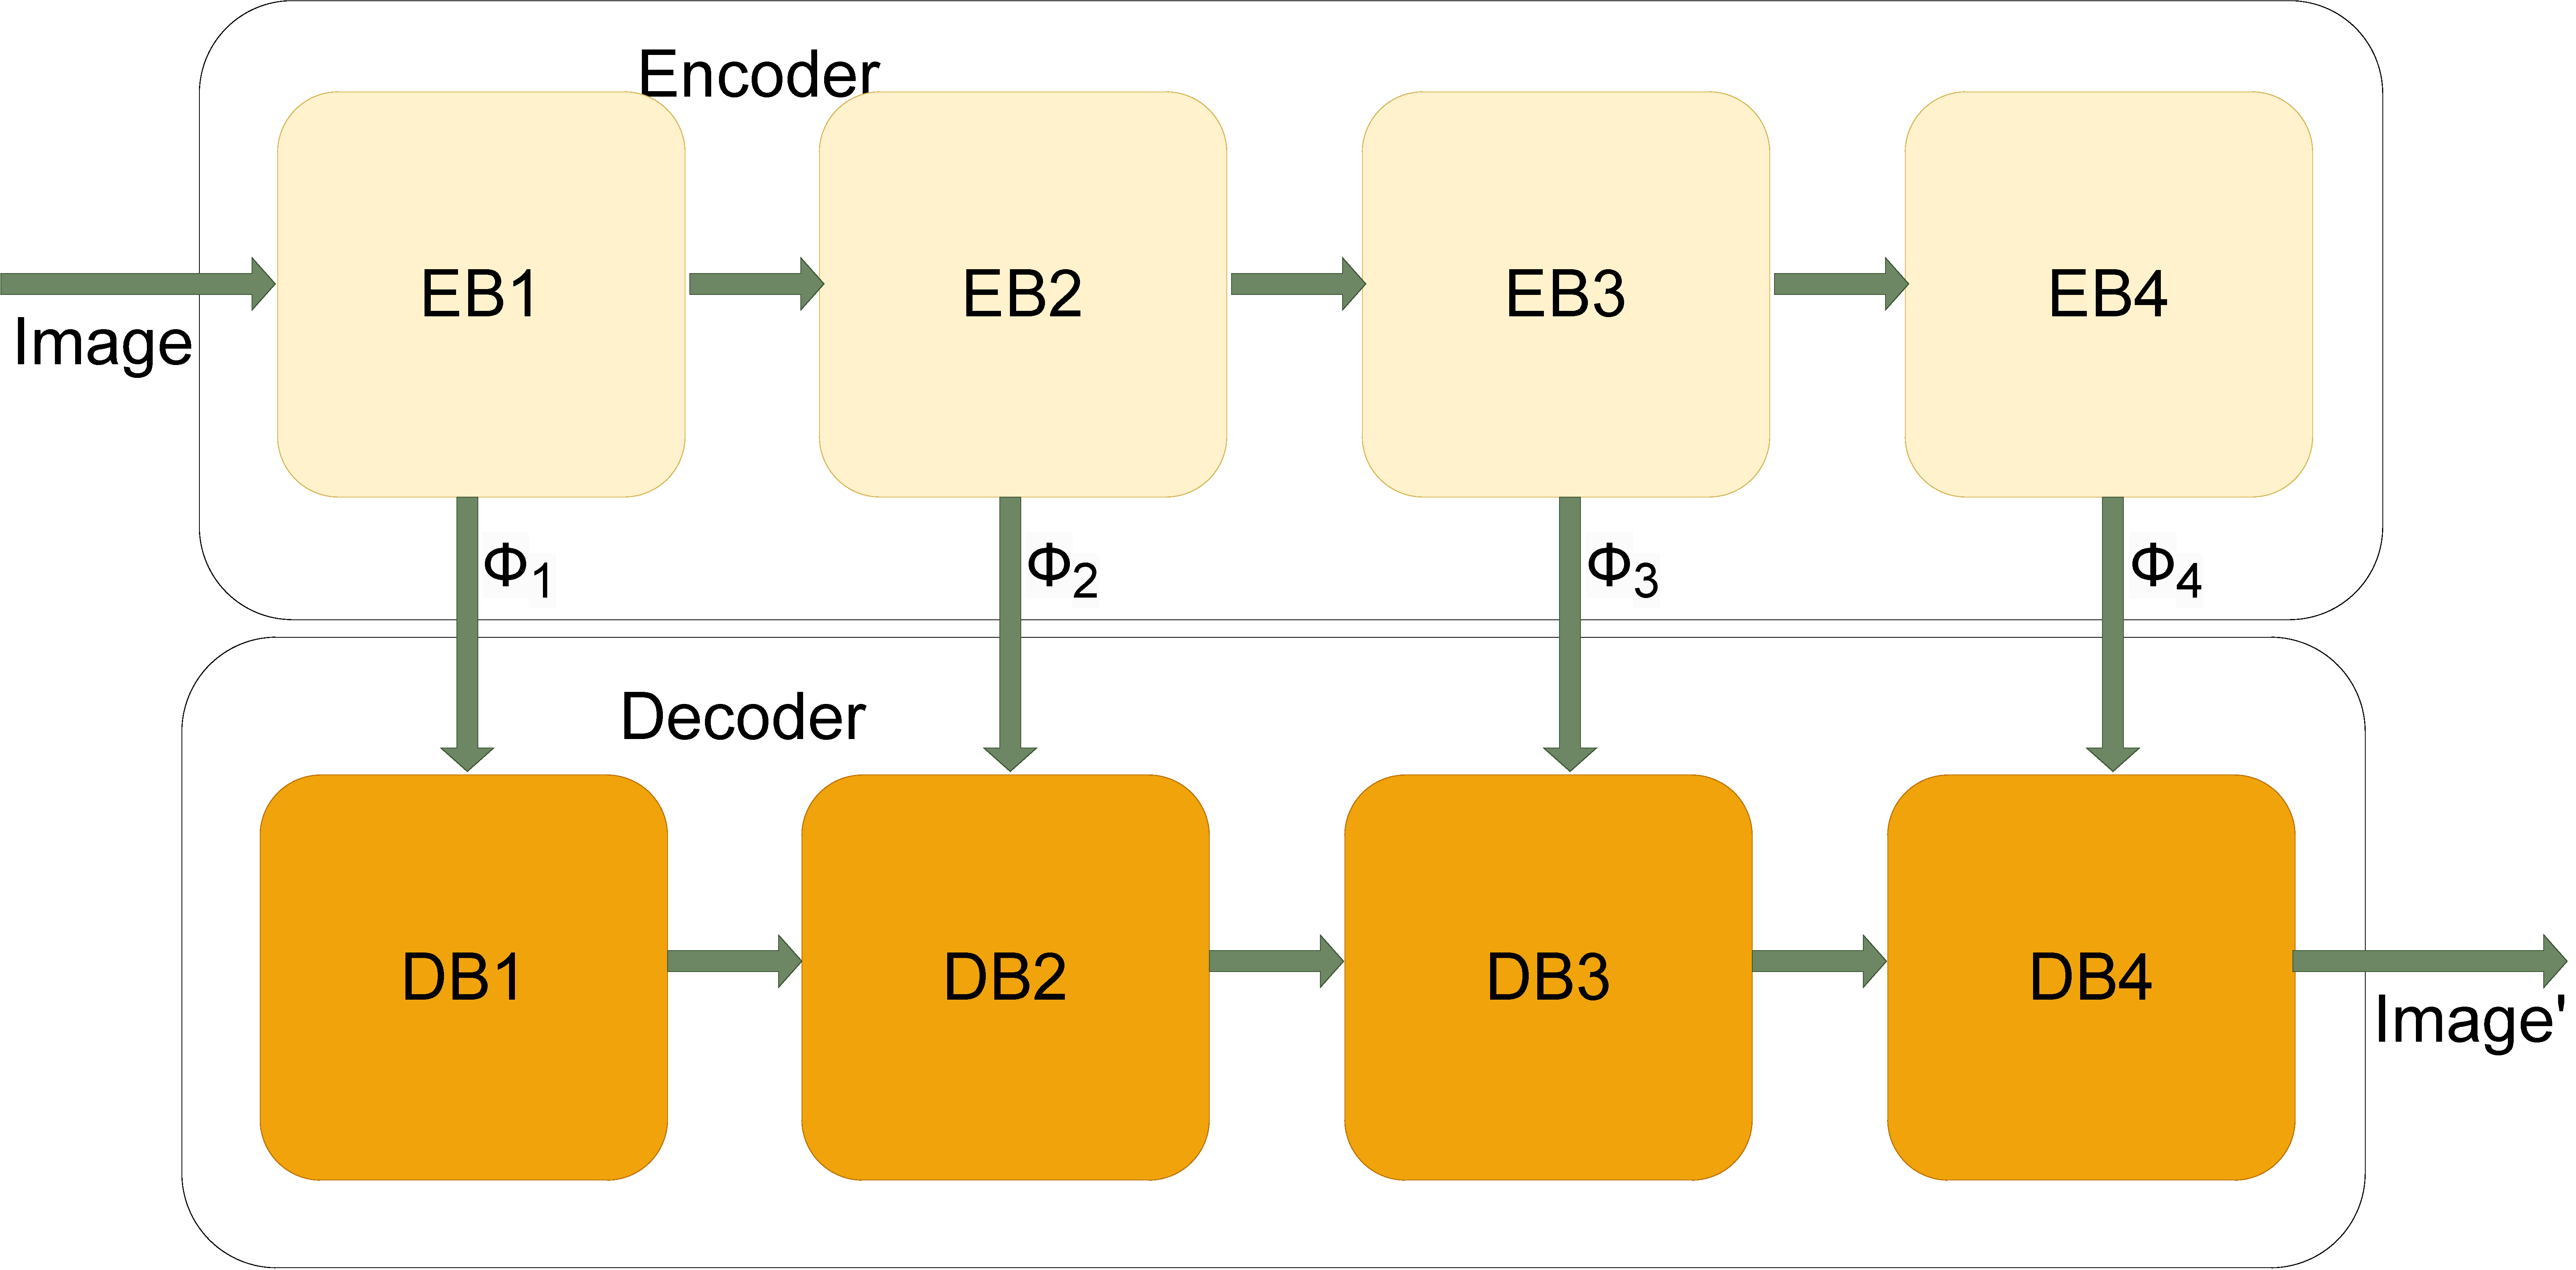
\includegraphics[width=0.4\textwidth]{imgs/stage1.pdf}
        \captionsetup{justification=raggedright,singlelinecheck=false}
        \caption{Block Diagram}
        \label{fig:ch3:stage1}
    \end{subfigure}
    \vspace{0.01cm}
    \begin{subfigure}[b]{\textwidth}
        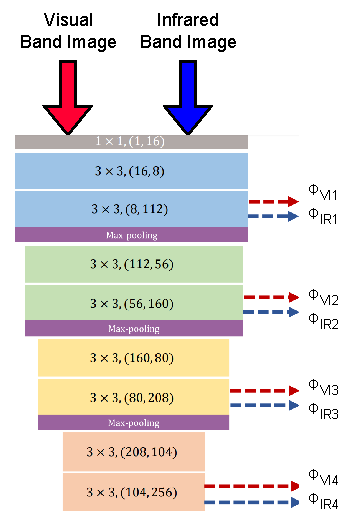
\includegraphics[width=0.4\textwidth]{imgs/encoder.pdf}
        \captionsetup{justification=raggedright,singlelinecheck=false}
        \caption{RFN-Nest \cite{li2021rfn} Encoder}
        \label{fig:ch3:encoder}
    \end{subfigure}
    \vspace{0.01cm}
    \begin{subfigure}[b]{\textwidth}
        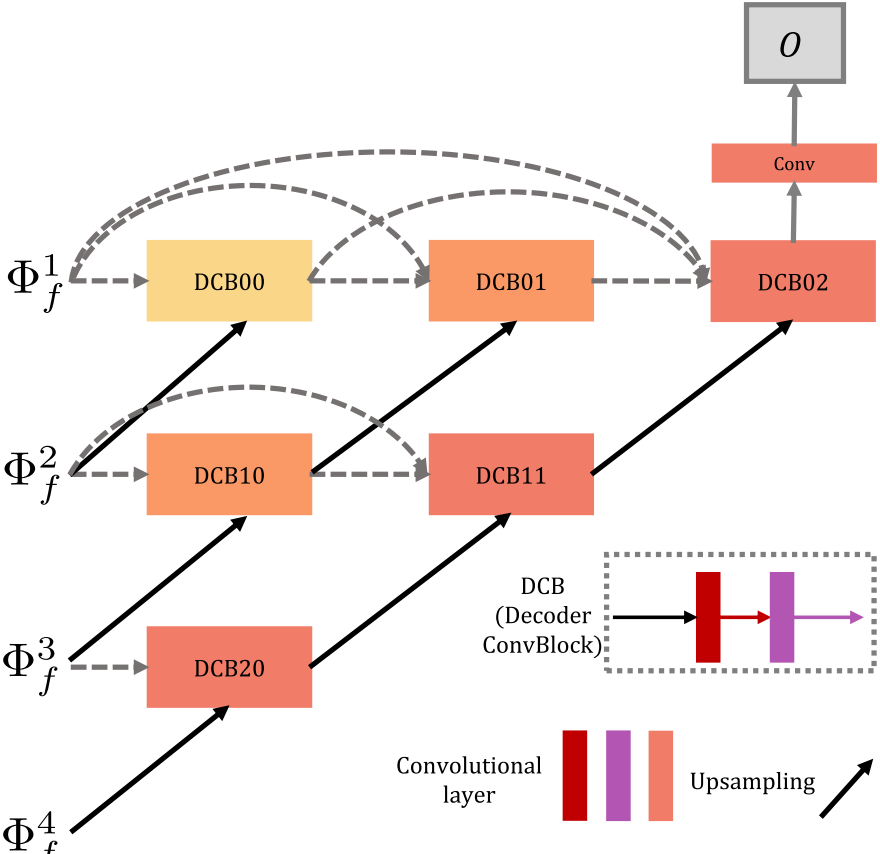
\includegraphics[width=0.4\textwidth]{imgs/decoder.png}
        \captionsetup{justification=raggedright,singlelinecheck=false}
        \caption{RFN-Nest \cite{li2021rfn} Decoder}
        \label{fig:ch3:decoder}
    \end{subfigure} 
    \caption{Stage 1 Configuration}
    \label{fig:ch3:stage1all}
\end{figure}

Training autoencoders presents a set of challenges that require careful consideration and effective solutions. One of the primary obstacles encountered is the vanishing or exploding gradients during backpropagation, which can hinder the convergence of the model. To overcome this, using activation functions like $ReLU$ and employing gradient clipping techniques can stabilize the training process. Another critical issue is overfitting, where the model becomes too specialized to the training data. Regularization methods such as $L1$ or $L2$ regularization and dropout can help prevent overfitting and improve generalization.

In the realm of autoencoders, choosing the right latent space dimension is crucial. A thorough hyperparameter search, including techniques like cross-validation, guides this selection. Autoencoders face challenges with multimodal data and computational demands, necessitating effective data preprocessing and optimization strategies.

Despite their capabilities, autoencoders may yield features lacking human interpretability. Techniques like activation maximization and feature visualization aid in deciphering model representations. Our approach adopts an autoencoder from RFN-Nest and DenseFuse, fine-tuning it on the MS-COCO and RoadScene datasets for robust feature extraction. Detailed in Section \ref{chp:results}, this staged training produces a proficient autoencoder. Examined on the TNO dataset, the findings illuminate potential applications and future directions for advancing image fusion techniques.

The initial phase of the training process involves instructing the encoder network to capture multi-scale deep features. Concurrently, the decoder network is also trained to reconstruct the input image, utilizing the aforementioned multi-scale deep features. The training framework of the auto-encoder network is depicted in Figure \ref{fig:ch3:rfnnest}. Distinguished from previous research, our feature extraction component integrates a down-sampling operation via max pooling, facilitating the extraction of deep features at various scales. These extracted multi-scale deep features are then fed into the decoder network for the purpose of reconstructing the input image. Leveraging short cross-layer connections ensures the comprehensive utilization of the multi-scale deep features in the image reconstruction process.

The loss function, denoted as $L_{ae}$, serves as the training criterion for the autoencoder network and is defined in the subsequent manner:

\begin{equation}\label{eq:aeloss}
    L_{ae} = L_{pixel} + \alpha  L_{SSIM}
\end{equation}

The terms $L_{pixel}$ and $L_{SSIM}$ refer to the pixel loss and the structural similarity (SSIM) loss, respectively, computed between the input and output images. The parameter $\alpha$ represents the trade-off parameter governing the balance between the contributions of $L_{pixel}$ and $L_{SSIM}$ meanwhile also it handles the order of magnitude difference in the overall loss function in Eq \ref{eq:aeloss}. 

\begin{equation}\label{eq:aelosspixel}
    L_{\text{pixel}} = \left\lvert \left\lvert\text{image}_{\text{output}} - \text{image}_{\text{input}} \right\rvert \right\rvert _{F}^{2}
\end{equation}

$L_{pixel}$ is defined in Eq \ref{eq:aelosspixel}. where $\left\lvert \left\lvert\text{.} \right\rvert \right\rvert _{F}$ denotes Frobenius norm. The Frobenius norm, denoted as $\|A\|_F$, is a matrix norm that measures the size or magnitude of a matrix $A$. For an $m \times n$ matrix $A$, the Frobenius norm is defined as the square root of the sum of the squares of all the elements of the matrix as in Eq \ref{eq:Frobenius}:

\begin{equation}\label{eq:Frobenius}
    \|A\|_F = \sqrt{\sum_{i=1}^{m} \sum_{j=1}^{n} |a_{ij}|^2}
\end{equation}

where $a_{ij}$ represents the element in the $i$th row and $j$th column of matrix $A$.

$L_{pixel}$ ensures that the reconstructed image closely resembles the original input image at the individual pixel level, imposing a constraint on the fidelity of pixel-wise information in the reconstruction process. This constraint helps to maintain fine-grained details and accuracy in the reconstructed image, ensuring that it retains the essential characteristics of the input image at a granular level. 

The second term in Eq \ref{eq:aeloss} is the SSIM loss $L_{SSIM}$ is defined as in Eq \ref{eq:ssimloss}:

\begin{equation}\label{eq:ssimloss}
    L_{SSIM} = 1- SSIM(image_{output},image_{input})
\end{equation}

where $SSIM(.)$ is the structural similarity measure \cite{ma2015perceptual} which quantifies the structural similarity of the two images. The structural similarity between Input and Output is constrained by
$L_{SSIM}$. The Structural Similarity Index (SSIM) is a widely used metric for evaluating the similarity between two images. It aims to capture not only the pixel-wise differences but also the structural information and perceptual quality of the images. The $SSIM(.)$ is formulated as in Eq \ref{eq:ssim} and Figure \ref{fig:ch3:ssim}.

\begin{equation}\label{eq:ssim}
\text{SSIM}(x, y) = \frac{{(2\mu_x\mu_y + C_1) \cdot (2\sigma_{xy} + C_2)}}{{(\mu_x^2 + \mu_y^2 + C_1) \cdot (\sigma_x^2 + \sigma_y^2 + C_2)}}
\end{equation}

where:
\begin{list}{}{}
    \item\(x\) and \(y\) represent the two images being compared.
    \item\(\mu_x\) and \(\mu_y\) are the local means of \(x\) and \(y\) respectively.
    \item\(\sigma_x^2\) and \(\sigma_y^2\) are the local variances of \(x\) and \(y\) respectively.
    \item\(\sigma_{xy}\) is the local covariance between \(x\) and \(y\).
    \item\(C_1\) and \(C_2\) are constants to stabilize the division with weak denominators. They are often set to small values, such as \(C_1 = (k_1 \cdot L)^2\) and \(C_2 = (k_2 \cdot L)^2\), where \(L\) is the dynamic range of pixel values, and \(k_1\) and \(k_2\) are constants typically set to small positive values.
\end{list}

The Structural Similarity Index ($SSIM$) is a metric that quantifies the similarity between two images, yielding values within the range of -1 to 1. A $SSIM(\bigodot,\bigodot)$ value of 1 denotes perfect similarity, indicating that the images share \textbf{same} characteristics in terms of luminance, contrast, and structure. Conversely, a value close to -1 signifies a substantial dissimilarity between the images. Notably, the $SSIM(\bigodot,\bigodot)$ index demonstrates a strong correlation with human perception of image quality, making it widely employed in diverse image processing and computer vision applications \cite{ma2015perceptual}.

The equation for $SSIM$ ($SSIM(.)$) in Eq. (\ref{eq:ssim}) constrains its output to the range of $[-1,1]$, which consequently bounds the $L_{SSIM}$ loss function (as defined in Eq. (\ref{eq:ssimloss})) to the interval $[0,2]$. In this context, lower values of $L_{SSIM}$ indicate better performance with respect to $SSIM$. In contrast, the $L_{pixel}$ loss is unbounded. To balance the impact of both $L_{pixel}$ and $L_{SSIM}$ during training, the trade-off parameter $\alpha$ in Eq. (\ref{eq:aeloss}) governs their relative magnitudes.

In short, the autoencoder depicted in Figure \ref{fig:ch3:encoder} is subjected to training using the MS-COCO dataset \cite{lin2014microsoft} and the RoadScene dataset \cite{xu2020aaai}. The training process is guided by the loss function presented in Eq. (\ref{eq:aeloss}). Comprehensive assessments of the autoencoder's performance are presented, encompassing both quantitative and qualitative evaluations. 

\subsection{Stage 2: Fusion Strategy Selection} \label{subsec:fusion}

\begin{figure}[htbp]
    \centering
    \begin{subfigure}[b]{\textwidth}
        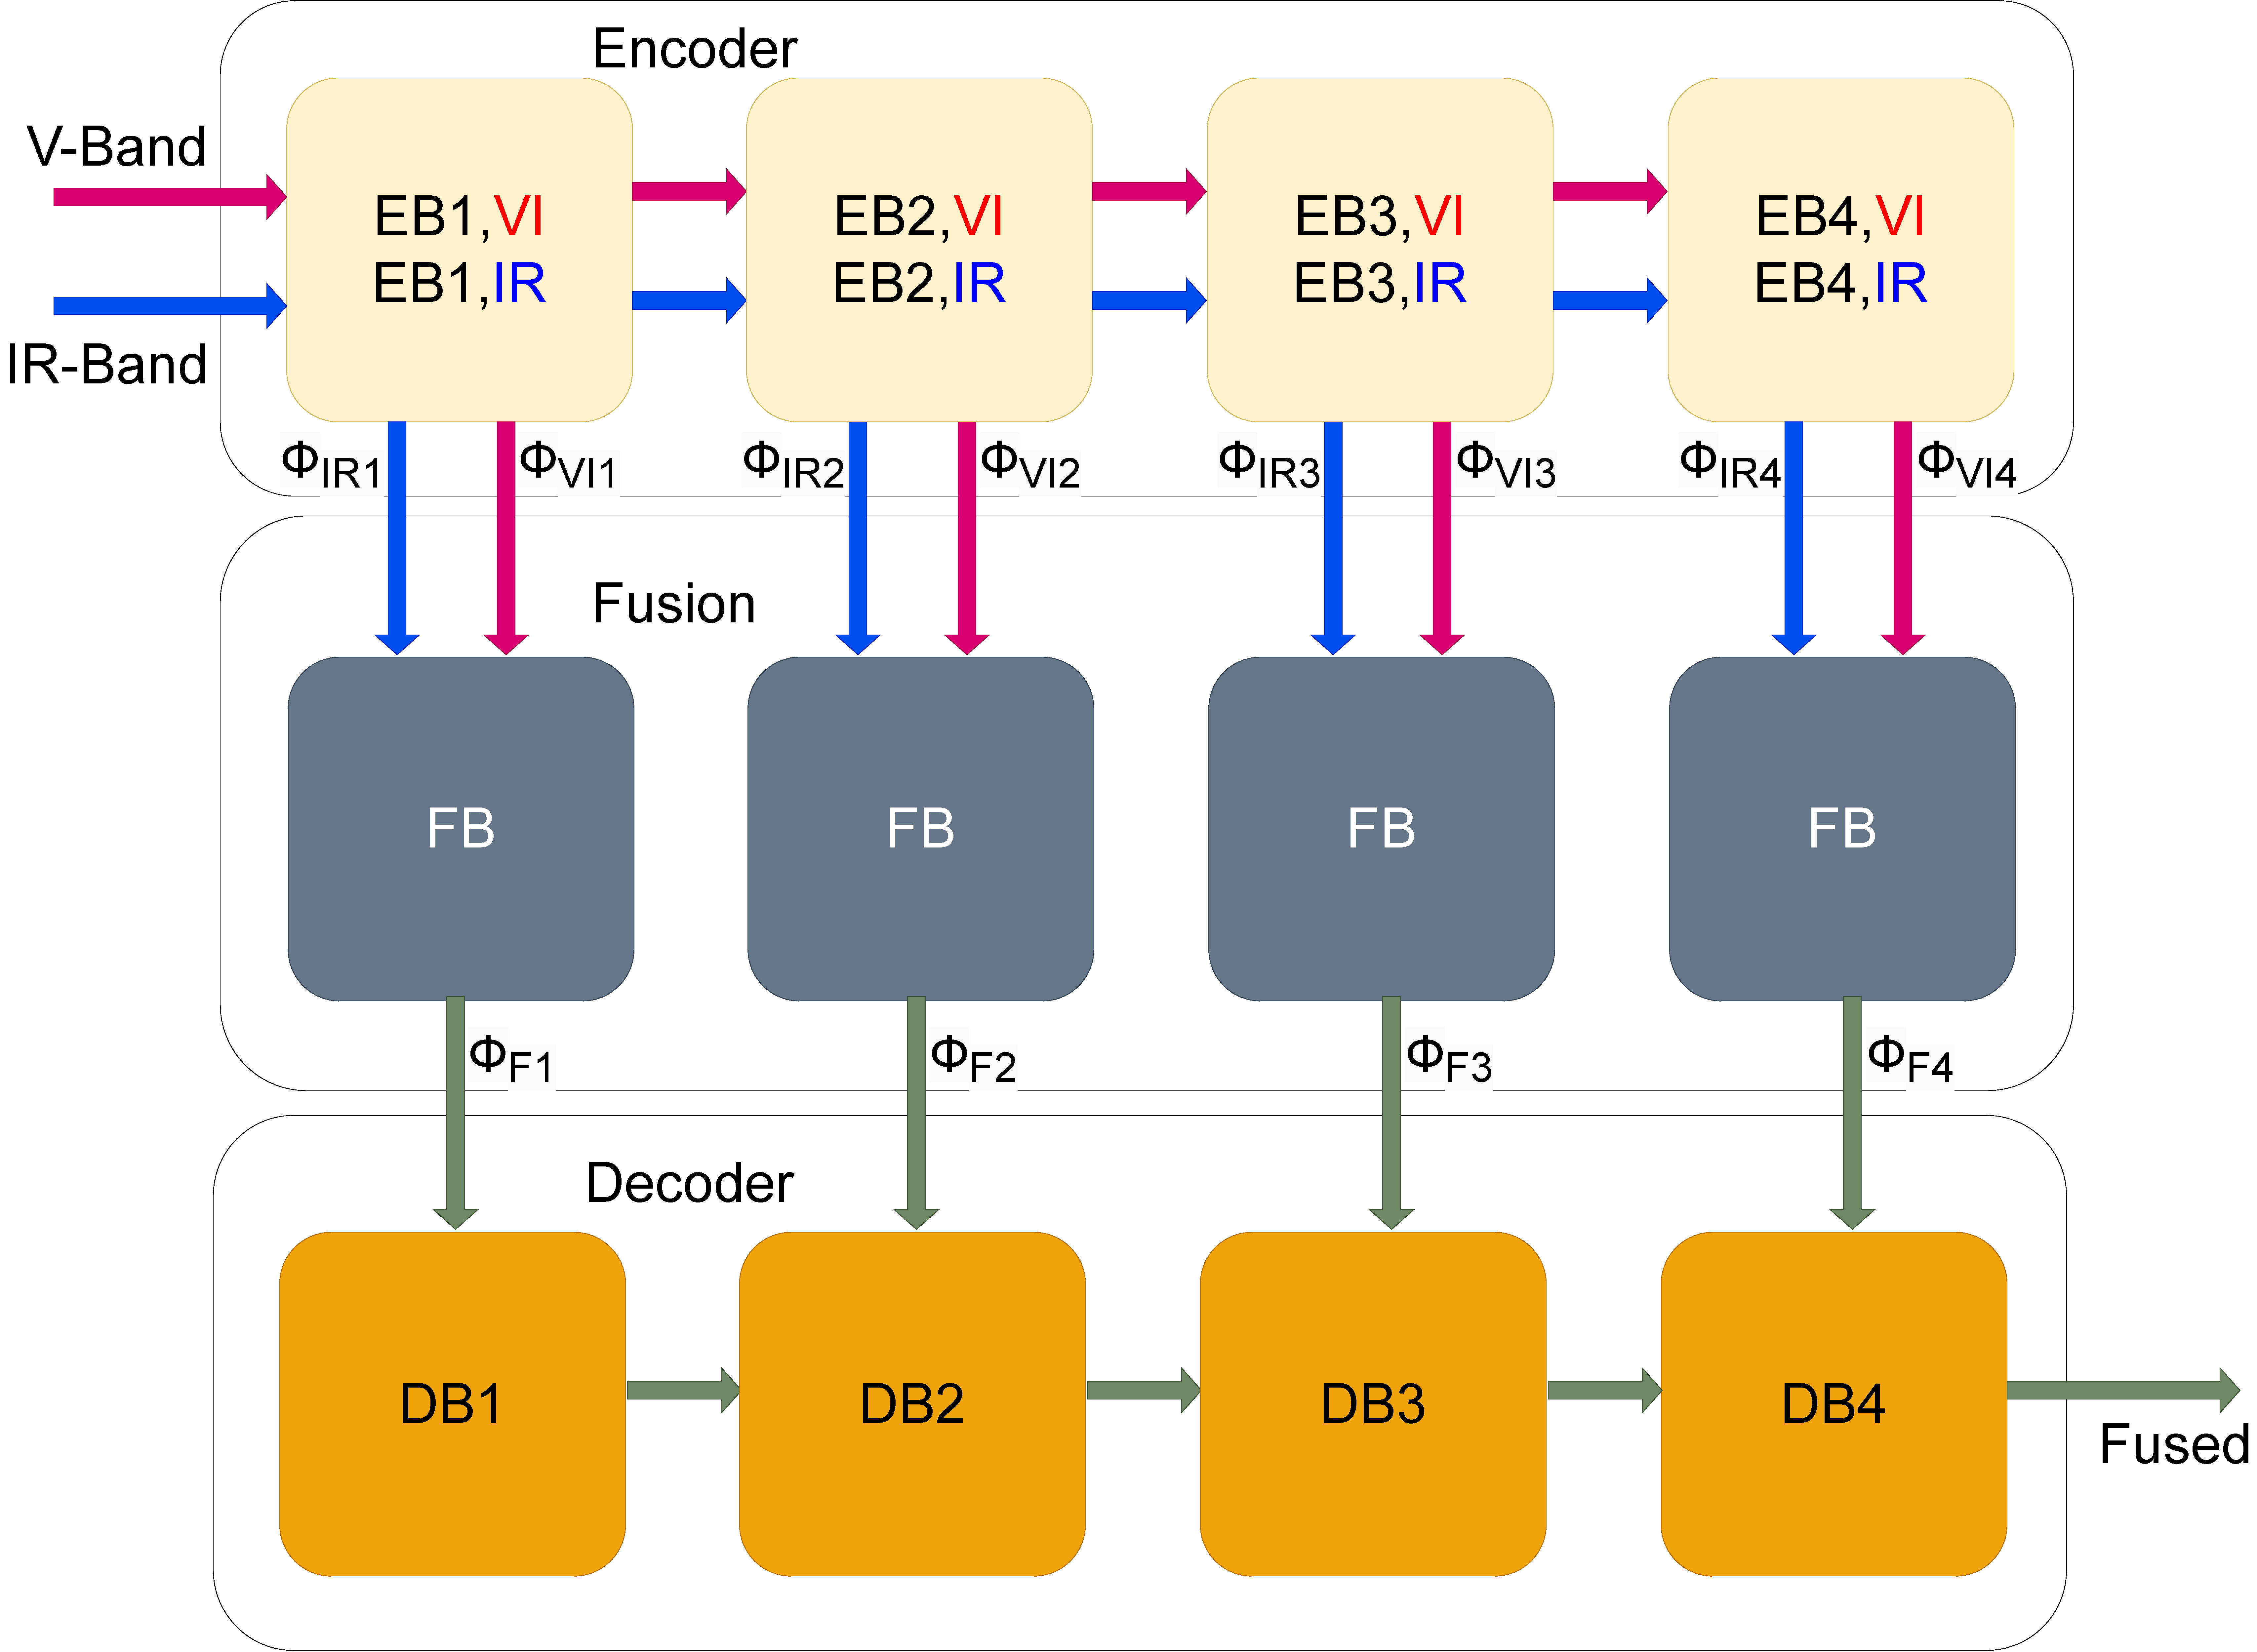
\includegraphics[width=0.5\textwidth]{imgs/stage2.pdf}
        \captionsetup{justification=raggedright,singlelinecheck=false}
        \caption{Block Diagram}
        \label{fig:ch3:stage2}
    \end{subfigure}
    \vspace{0.01cm}
    \begin{subfigure}[b]{\textwidth}
        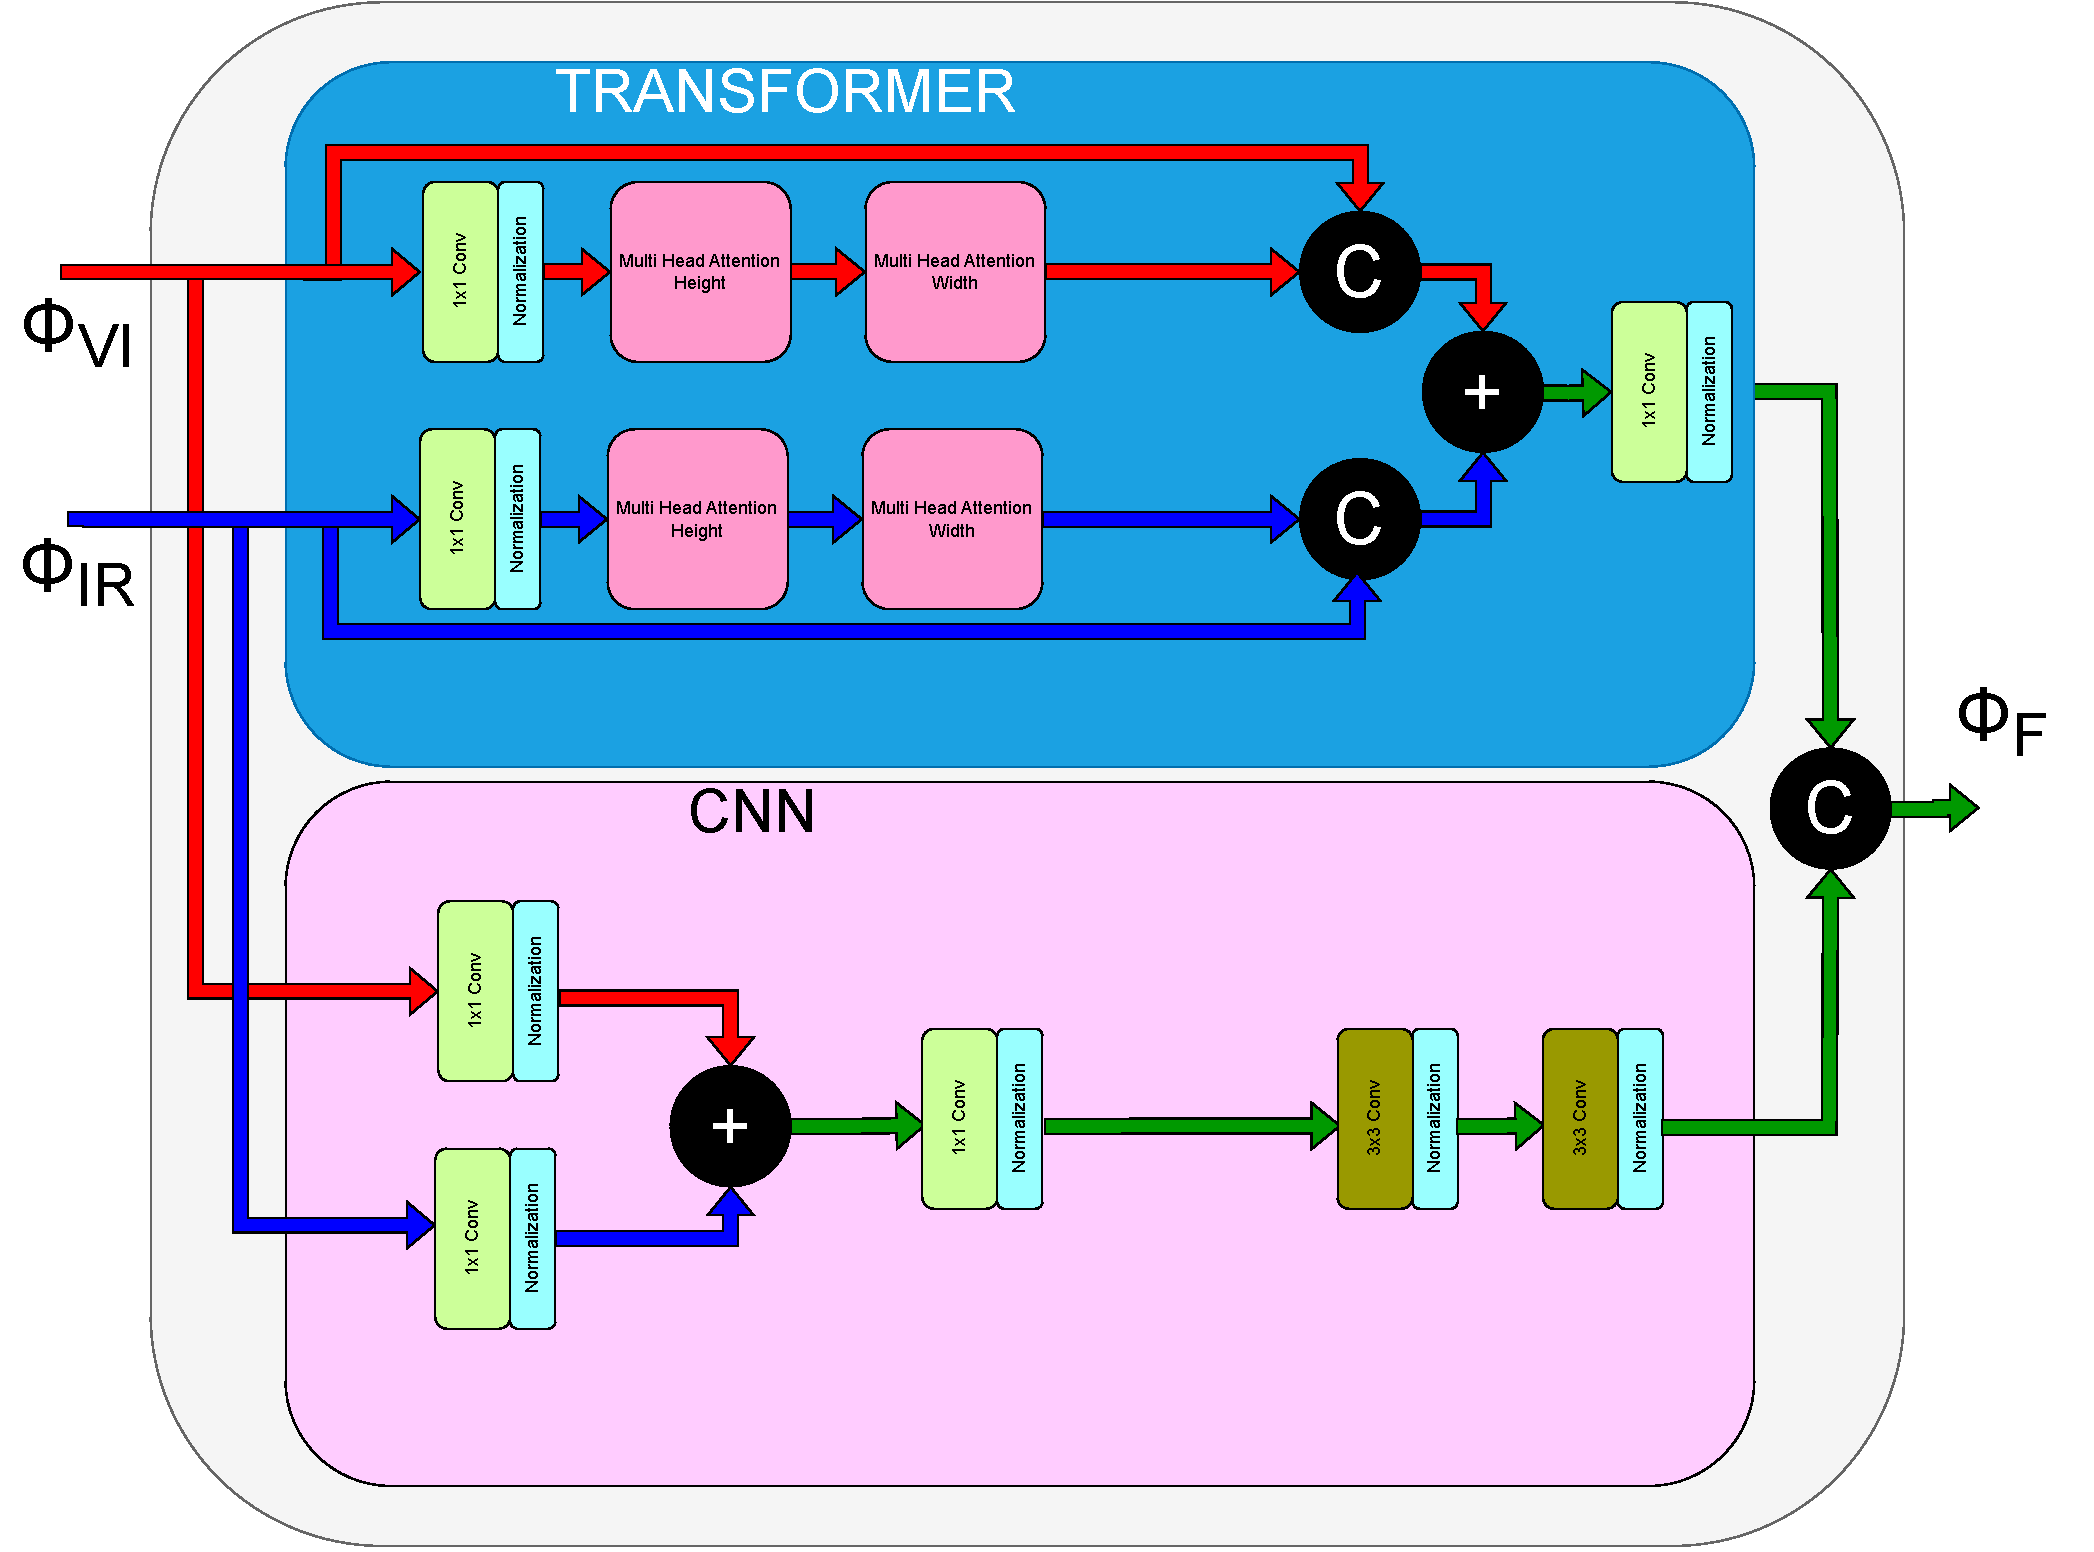
\includegraphics[width=0.5\textwidth]{imgs/transformerblok.pdf}
        \captionsetup{justification=raggedright,singlelinecheck=false}
        \caption{Fusion Block}
        \label{fig:ch3:fusion}
    \end{subfigure}
    \caption{Stage 2 Configuration}
    \label{fig:ch3:stage2all}
\end{figure}

The process involved in accurately extracting multi-scale feature maps, coupled with the decoding and reconstruction of the original image as illustrated in Figure \ref{fig:ch3:stage1}, has been previously discussed. This process is primarily concerned with the extraction of complex features at various scales which are intrinsic to image data. The essence of multi-scale feature extraction is to gather spatially diverse information from the image at different resolutions, thereby allowing for a more robust representation of the image data.

Presently, the emphasis will shift to the application of separate encoders for the extraction of multi-scale features from both visual and infrared band images. The process entails the deployment of these encoders, each uniquely purposed for their respective image band. This is important as different image bands often contain distinct but complimentary information. For instance, \textbf{the visual image band, which relies on the visible light spectrum, presents color and texture details, while the infrared band, capturing non-visible light, provides thermal information}.

The outputs from these separate encoders are then merged into a single multi-scale feature map with fusion block depicted in Figure \ref{fig:ch3:fusion} per scale. This fusion process is a crucial step as it combines diverse features from different bands, enhancing the feature representation. It allows the model to leverage the strengths of each band, thereby improving the overall effectiveness of the feature extraction process.

Following the fusion, the resulting multi-scale feature maps are subsequently decoded, leading to the reconstruction of the original image, as depicted in Figure \ref{fig:ch3:highlevel}. It is important to note that this decoding phase does not merely entail the generation of a visually coherent image. Rather, it reconstructs an image that encapsulates the combined information from both bands. In essence, the reconstructed image, though visually similar to the original, carries a much richer set of features, potentially paving the way for more accurate subsequent analyses or processes.

Conventional Convolutional Neural Network (CNN) based techniques facilitate image fusion through the amalgamation of local features. However, a significant limitation inherent to these methods is their lack of consideration for the global context that permeates an image. In an attempt to circumvent this limitation, transformer-based models have been introduced, which capitalise on the self-attention mechanism to effectively model the global context.

The development of an innovative approach that synthesises transformer-based models with CNNs is thus postulated. This approach strives to account for local features at multiple scales, paying careful attention to both local and global contexts. As articulated in Section \ref{sec:model}, the method that is proposed adopts a bi-phase training protocol.

The first stage of this training protocol necessitates the use of an auto-encoder to extract deep, multi-scale features. In the subsequent stage, these multi-scale features are blended via a fusion strategy that innovatively combines CNNs with Transformers. Comprising a CNN and a transformer branch, the combined fusion blocks capably capture both local and global context features.

Further experimentation with this method was undertaken on a multitude of benchmark datasets, as illustrated in Section \ref{chp:results}. Comparative metrics, as specified in Section \ref{subsec:metrics}, revealed that the method proposed outperformed many existing fusion algorithms. The results demonstrated that the combined CNN-Transformer fusion strategy was effective in capturing a broader context, leading to superior performance in various comparative metrics. 

This method's success lies in its ability to leverage the strengths of both CNNs and Transformer models, providing a comprehensive view of an image by capturing both local and global contexts. The strategy's robustness, combined with its efficiency, heralds a new direction for further developments in the field of image fusion. Used combined fusion block details can be seen at Figure \ref{fig:ch3:fusionhighlevel}.


The fusion network, illustrated in Figure \ref{fig:ch3:fusiondetailed}, is characterised by its dual-branch design, which consists of a spatial branch and a transformer branch. The spatial branch integrates convolution layers and a bottleneck layer, specifically tailored to distil local feature representations. Conversely, the transformer branch employs an axial attention-based transformer block to capture the global context embedded within the input data. 

The Local Feature Fusion block within the spatial branch operates in a relatively straightforward manner, focusing on exploiting spatial dependencies in the data to extract intricate local features. The structure and functionality of this branch can be observed in Figure \ref{fig:ch3:fusiondetailed}. 

Meanwhile, for the transformer branch, two alternatives can be considered for attention mechanism deployment: self-attention and axial-attention.

The self-attention mechanism is a strategic process that correlates disparate tokens within a singular sequence to generate a representative sequence. It is an effective method for modelling dependencies without regard to their position in the input. Consider an input feature tensor $x \in \mathbb{R}^{C_{\text{in}} \times H \times W}$ and output feature tensor $y \in \mathbb{R}^{C_{\text{out}} \times H \times W}$. Here, $C_{in}$ and $C_{out}$ respectively denote the quantity of input and output channels, while $H$ and $W$ are indicative of the tensor's height and width, respectively. 

The self-attention mechanism can be mathematically formulated as in Eq \ref{eq:selfattention}:

\begin{equation} \label{eq:selfattention}
\begin{split}
    Q &= xW_{Q}\\
    K &= xW_{K}\\
    V &= xW_{V}\\
    A &= \text{softmax}\left(\frac{QK^{T}}{\sqrt{d}}\right)\\
    y &= AV
\end{split}
\end{equation}

In these equations, $W_Q$, $W_K$, and $W_V$ are weight matrices that are learned. $Q$, $K$, and $V$ symbolise the query, key, and value, which are derived from the input tensor $x$. After obtaining these matrices, the attention scores $A$ are calculated using a softmax function applied to the dot product of $Q$ and $K^T$, which is further scaled by $1/\sqrt{d}$. The output feature tensor $y$ is then obtained by multiplying the attention scores with the value matrix $V$. 

Alternatively, the axial-attention mechanism, as presented by Ho et al. \cite{ho2019axial}, offers a unique approach to sequence processing. This mechanism, a variant of self-attention, is characterised by its improved computational efficiency. In axial attention, the application of self-attention is executed sequentially over the axes of the feature map's height, followed by the width. This approach significantly reduces computational complexity, thus fostering more efficient operations.

A noteworthy contribution to the axial attention mechanism was proposed by Wang et al. \cite{wang2020axial}, who introduced a learnable positional embedding to the query, key, and value of axial attention. This addition enhances the sensitivity of the affinities to positional information, further improving the performance of the mechanism. These positional embeddings are considered parameters that are learned in conjunction with the training process.

Considering an input $x$, the self-attention computation along the height axis can be formulated as presented in Eq \ref{eq:axialH}, and along the width axis as shown in Eq \ref{eq:axialW}:

\begin{equation} \label{eq:axialH}
    \begin{split}
        y_{ij} = \sum_{h=1}^{H} \text{softmax}\left(q_{ij}^{T}k_{ih} + q_{ij}^{T} r_{ih}^q + k_{ij}^{T} r_{ih}^k\right)
    \end{split}
\end{equation}

Here, $r^q$, $r^k$, and $r^v$ $\in \mathbb{R}^{H \times H}$ represent the positional embeddings for the height axis. 

\begin{equation} \label{eq:axialW}
    \begin{split}
        y_{ij} = \sum_{w=1}^{W} \text{softmax}\left(q_{ij}^{T} k_{iw} + q_{ij}^{T} r_{iw}^q + k_{ij}^{T} r_{iw}^k\right)
    \end{split}
\end{equation}

Here, $r^q$, $r^k$, and $r^v$ $\in \mathbb{R}^{W \times W}$ denote the positional embeddings for the width axis.

The axial attention mechanism, employing specific equations for height and width axes, as depicted in Eq \ref{eq:axialH} and Eq \ref{eq:axialW}, respectively, contributes to the efficacy of a self-attention model, visually illustrated in Figure \ref{fig:ch3:fusiondetailed}. This mechanism proves versatile in learning meaningful representations, demonstrating applicability across diverse fields. Constructing resilient axial attention transformer architectures requires a fusion of theoretical insights and practical approaches, a crucial combination for proficiently addressing complex real-world challenges.

Addressing potential issues, axial attention transformers, like other transformer-based models, may encounter difficulties with long-range dependencies, quadratic time complexity, lack of interpretability, overfitting, and training stability. Solutions involve introducing position encodings, efficient attention variants, interpretability techniques, regularization, and gradient clipping. Our approach involves adopting an axial attention transformer as the base model in the Image Fusion Transformer \cite{vs2022image}, fine-tuned on the RoadScene \cite{xu2020aaai} dataset, resulting in a pretrained model adept at capturing essential features. In summary, the dual-branch design of the network, incorporating a spatial branch for local features and a transformer branch for global context, provides a comprehensive feature representation, making it a promising tool for various applications.

In the initial training phase, the focus is on empowering the encoder network to capture multi-scale deep features. Simultaneously, the decoder network is trained to reconstruct the input image by leveraging these multi-scale deep features, extracted by the trained encoder network. The autoencoder network's structure and training scheme are depicted in Figure \ref{fig:ch3:encoder}, illustrating the coordinated learning process.

Moving forward to the second phase, detailed in Section \ref{sec:model}, the training regimen introduces the fusion block between the encoder and decoder, illustrated in Figure \ref{fig:ch3:fusionhighlevel}. This crucial step prompts a reassessment of the initial loss function employed during the autoencoder training stage, specified by Eq \ref{eq:aeloss} in Section \ref{subsec:aeloss}. The objective is to scrutinize the effectiveness of this loss function for the current stage of training, ensuring its alignment with the fusion block integration.

The fusion loss function, $L_{fuse}$, can be formulated as in Eq \ref{eq:fuseloss}:

\begin{equation}\label{eq:fuseloss}
    L_{fuse} = L_{pixel} + \alpha  L_{structure}
\end{equation}

This fusion loss function aims to balance the contribution from pixel-level losses, denoted as $L_{feature}$, and structural similarity losses, $L_{structure}$, modulated by a trade-off factor, $\alpha$. This mathematical construct becomes critical in the context of our analysis and potential modification of the loss function used in the preceding training stage, thereby introducing an additional degree of intricacy to the model's optimization procedure.

It is clear that the autoencoder loss function is insufficient to meet the needs of the fusion strategy. This is due to the following reasons:

\begin{itemize}
    \item $L_{fuse} = 0$ in Eq \ref{eq:fuseloss} signifies an optimal fusion condition, excluding the overfitting case. This implies that both $L_{feature}$ in Eq \ref{eq:aelosspixel} and $L_{structure}$ in Eq \ref{eq:ssimloss} must independently be equal to zero.
    \item $L_{feature} = 0$ in Eq \ref{eq:aelosspixel} occurs only when the input and output images are identical.
    \item Likewise, $L_{structure} = 0$ in Eq \ref{eq:ssimloss} is achieved only when the input and output images are identical.
\end{itemize}

To ensure $L_{fuse} = 0 $ in Eq \ref{eq:fuseloss} corresponds to an optimal fusion scenario, the definitions of $L_{structure}$ and $L_{feature}$ must be updated as shown in Eq \ref{eq:fusepixelloss} and Eq \ref{eq:fusessimloss} respectively. The following constraints need to be considered:

\begin{enumerate}
    \item The fused image should have a higher resemblance to the visual band image while maintaining the global context from the infrared band image almost identical to the visual band image. As a result, $L_{structure}$ must be computed for both input visual and infrared band images, ideally but not necessarily favoring the visual band image.
    \item The pixel values of the fused image should closely match the visual band image due to its compatibility with human vision. Hence, $L_{feature}$ must be calculated on both input visual and infrared band images.
\end{enumerate}

The SSIM loss $L_{structure}$ is then defined as:

\begin{equation} \label{eq:fusessimloss}
    L_{structure} = \left[1- SSIM(I_{fused},I_{visual})\right]^2 + \left[1- SSIM(I_{fused},I_{infrared})\right]^2
\end{equation}

Here, $I_x$ represents $image x$ and $SSIM(.)$ is the structural similarity measure \cite{ma2015perceptual} given in Eq \ref{eq:ssim}. The redefined $L_{structure}$ is capable of measuring the similarity of the fused image to both visual and infrared images, and is limited to the interval $(0,8]$.

The pixel-wise loss $L_{feature}$ can be formulated as:

\begin{equation} \label{eq:fusepixelloss}
    L_{feature} = \sum_{m=1}^{M} \omega^m \left\lvert \left\lvert \phi_f^m - \left(\omega_{vi}\phi_{vi}^{m} + \omega_{ir}\phi_{ir}^{m}\right) \right\rvert \right\rvert _{F}^{2}
\end{equation}

Here, $M$ refers to the number of scales for deep feature extraction, while $f$, $vi$, and $ir$ denote the fused image, the input visual band image, and the input infrared band image respectively. $\omega^m$, $\omega_{vi}$, and $\omega_{ir}$ represent trade-off parameters employed to harmonize the magnitudes of the losses. $\phi_{x}^{m}$ corresponds to the feature maps of $image x$, which could be either the input or output feature maps of the fusion block, as depicted in Figure \ref{fig:ch3:stage2all}.

This loss function restricts the fused deep features to preserve significant structures, thereby enriching the fused feature space with more conspicuous features and preserving detailed information.